%!TEX program = xelatex
%%%%%%%%%%%%%%%%%%%%%%%%%%%%%%%%%%%%%%%%%
% Short Sectioned Assignment
% LaTeX Template
% Version 1.0 (5/5/12)
%
% This template has been downloaded from:
% http://www.LaTeXTemplates.com
%
% Original author:
% Frits Wenneker (http://www.howtotex.com)
%
% License:
% CC BY-NC-SA 3.0 (http://creativecommons.org/licenses/by-nc-sa/3.0/)
%
%%%%%%%%%%%%%%%%%%%%%%%%%%%%%%%%%%%%%%%%%

%----------------------------------------------------------------------------------------
%	PACKAGES AND OTHER DOCUMENT CONFIGURATIONS
%----------------------------------------------------------------------------------------

\documentclass[paper=a4, fontsize=11pt]{scrartcl} % A4 paper and 11pt font size
\usepackage{xeCJK}
\usepackage[T1]{fontenc} % Use 8-bit encoding that has 256 glyphs
\usepackage{fourier} % Use the Adobe Utopia font for the document - comment this line to return to the LaTeX default
\usepackage[english]{babel} % English language/hyphenation
\usepackage{amsmath,amsfonts,amsthm} % Math packages
\usepackage{lipsum} % Used for inserting dummy 'Lorem ipsum' text into the template
\usepackage{enumerate}
\usepackage{sectsty} % Allows customizing section commands
\allsectionsfont{\normalfont\scshape} % Make all sections centered, the default font and small caps

\usepackage{fancyhdr} % Custom headers and footers
\pagestyle{fancyplain} % Makes all pages in the document conform to the custom headers and footers
\fancyhead{} % No page header - if you want one, create it in the same way as the footers below
\fancyfoot[L]{} % Empty left footer
\fancyfoot[C]{} % Empty center footer
\fancyfoot[R]{\thepage} % Page numbering for right footer
\renewcommand{\headrulewidth}{0pt} % Remove header underlines
\renewcommand{\footrulewidth}{0pt} % Remove footer underlines
\setlength{\headheight}{13.6pt} % Customize the height of the header

%\numberwithin{equation}{section} % Number equations within sections (i.e. 1.1, 1.2, 2.1, 2.2 instead of 1, 2, 3, 4)
\numberwithin{figure}{section} % Number figures within sections (i.e. 1.1, 1.2, 2.1, 2.2 instead of 1, 2, 3, 4)
\numberwithin{table}{section} % Number tables within sections (i.e. 1.1, 1.2, 2.1, 2.2 instead of 1, 2, 3, 4)

\setlength\parindent{0pt} % Removes all indentation from paragraphs - comment this line for an assignment with lots of text

\usepackage{bm}
\usepackage{algorithm}
\usepackage{algorithmic}

%----------------------------------------------------------------------------------------
%	TITLE SECTION
%----------------------------------------------------------------------------------------

\newcommand{\horrule}[1]{\rule{\linewidth}{#1}} % Create horizontal rule command with 1 argument of height

\title{	
\normalfont \normalsize 
\textsc{Zhiyuan College, Shanghai Jiao Tong University} \\ % Your university, school and/or department name(s)
\horrule{0.5pt} \\[0.4cm] % Thin top horizontal rule
\huge CS 225: Probability and Computing Homework 3 \\ % The assignment title
\horrule{2pt} \\ % Thick bottom horizontal rule
}

\author{
\normalsize
	Zihao Ye
} % Your name

\date{\normalsize\today} % Today's date or a custom date

\newtheorem{claim}{Claim}

\begin{document}

\maketitle % Print the title

\section*{Problem 1}
\begin{enumerate}[(a)]
	\item 
	\begin{proof}
	假设$p$为gambler赢的概率.

	可以估计出$E[T]$的上界:$E[T]\leq (a+b)2^{a+b}$(将$\{X_n\}$每$a+b$个分为一段, 用geometry distribution的期望计算)有限.

	那么由\textit{Wald's Equation}, 有
	$$pb + (1-p)\cdot-a = E\left[\sum_{i=1}^{T}X_i\right] = E[T]E[X_i] = 0 $$

	解得$p = \frac{a+b}{a}$.

	如果要写成利用\textit{O.S.T}的证明, 令$Y_t=\sum\limits_{i=1}^{t}\left(X_i - E[X_i]\right)$, 则$Y_t$是一个martingale w.r.t $X_0, X_1, \cdots$, 由\textit{O.S.T}得$0 = E[Y_T]$.
	\end{proof}
	\item
	\begin{proof}
	设$X_i$为第$i$次抛硬币的随机变量, $X_i = 1$时为正, $X_i = -1$时为负, 特别的, 令$X_0 = 0$.

	定义如下$Z_t$, $Z_{t}$由$X_1, X_2, \cdots, X_{t}$完全决定.

	设$Y_t = \sum\limits	_{i=1}^{t}X_i$即进行完$t$轮之后的$\#HEAD - \#TAIL$, 令
	$$Z_t = 
	\left\{\begin{array}{ll}
	(Y_t - b)(Y_t + a) - t 	& \forall i\in[t - 1] Y_{i} \in (a, b)\\
	Z_{t-1} 				& \exists i\in[t - 1] Y_{i} \geq b \textrm{ or } Y_{i} \leq -a 
	\end{array}\right.$$ 
	则可以证明$E[Z_t\mid X_1, X_2, \cdots, X_{t-1}] = Z_{t-1}$, 因此$Z_0, Z_1, \cdots$是关于$X_0, X_1, \cdots$的martingale.

	由上一问可知$E[T]$有限.

	由于$E[|Z_{t+1}-Z_{t}\mid X_0, \cdots, X_t]\leq 1 + (a+b)^2$是个常数, 由\textit{O.S.T}得:

	$$
 		-E[T] = E[Z_T] = E[0] = -ab \Longrightarrow E[T] = ab
 	$$
	\end{proof}

\end{enumerate}

\section*{Problem 2}
	设某次flip的clause中变量为$\sigma_i, \sigma_j$, 则$\sigma_i\not= \pi_i \textrm{ or } \sigma_j \not= \pi_j$.

	因此设$D^{(1)}_i$为进行第$i$次flip时$\sigma$与$\pi$的\textit{Hamming distance}.
	$$\textit{Pr}\left[D^{(1)}_{i + 1} - D^{(1)}_{i} = -1\right] \geq \frac{1}{2} $$

	可将此过程设为在一维空间上$[0, n]$区间内进行的随机游走, 且初始位置未知, 每次向$0$方向走一步的概率$\geq\frac{1}{2}$. 停时定义为$T$时刻$\sigma$与某个合法的$\pi$重合, 若$D^{(1)}_t=0, T\leq t$, 但$D^{(2)}_T$不一定$=0$, 设此过程为$\mathfrak{M}_1$.

	考虑一个类似的问题, 在$[0, 2n]$区间内进行随机游走, 初始位置在$[0, n]$之间与$\mathfrak{M}_1$的初始位置相同, 停时为在$T$时刻到达$0$或$2n$, 设此过程为$\mathfrak{M}_2$.

	我们考虑coupling, 产生一系列$[0,1]$中独立均匀分布的随机变量$\{X_i\}$, 则在$\mathfrak{M}_1$中:

	$$ D^{(1)}_{i+1} - D^{(1)}_{i} = 
	\left\{
	\begin{array}{ll}
	-1  & X_i\leq \textit{Pr}\left[D^{(1)}_{i+1} - D^{(1)}_{i} = -1\right] \\
	1	& \textrm{otherwise}
	\end{array}
	\right.
	 $$

	在$\mathfrak{M}_2$中:

	$$ D^{(2)}_{i+1} - D^{(2)}_{i} =
	\left\{
	\begin{array}{ll}
	-1 & \left(D^{(2)}_i \leq n \textrm{ and } X_i\leq \frac{1}{2} 
		 \right) \textrm{ or }
		 \left(D^{(2)}_i > n    \textrm{ and } X_i\geq \frac{1}{2}
		 \right) \\
	1  & \textrm{otherwise} 
	\end{array}
	\right. 
	$$

	则可以证明此时$Pr\left[D^{(2)}_{i+1} - D^{(2)}_{i} = -1 \right] = \frac{1}{2}$且两两独立.

	同时有:$$\min\left\{2n - D^{(2)}_{i}, D^{(2)}_{i}\right\} \geq D^{(1)}_{i} $$

	设$T_2$为过程$\mathfrak{M}_2$的停时, 由于$\min\left\{2n - D^{(2)}_{T_2}, D^{(2)}_{T_2}\right\} = 0 \geq D^{(1)}_{T_2}$, 因此此时有$D^{(1)}_{T_2} = 0, T_1\leq T_2$.

	由\textit{PROBLEM 1}的结论, $E[T_2] = D^{(1)}_0\left(2n - D^{(1)}_0\right) = n ^ 2 - \left(D^{(1)}_0 - n\right)^2$.

	由此得出$E[T_1] \leq n^2 = O(n^2)$, 要使得准确率$\geq 99\%$, 则设一个此算法的flip次数上限$t=100n^2$:

	$$\textit{Pr}\left[T_1 \geq t\right] \leq \frac{E[T_1]}{t} \leq 0.01 $$ 

\section*{Problem 3}
	固定$v$, 构造一个circuit如下:

	\begin{eqnarray*}
	R_{u,v} & = & c_{uv} \\
	\forall u\in V, C^{-}_u  & = & d(u) \\
	C^{+}_v & = & 2m 
	\end{eqnarray*}
	
	根据基尔霍夫定律和安培定律可以写出如下等式:

	\begin{eqnarray*}
		d(u) & = & \sum_{uw\in E} C_{u\rightarrow w} \\
			 & = & \sum_{uw\in E} \frac{\varphi_{u,w}}{R_{u,w}} \\
			 & = & \sum_{uw\in E} \frac{1}{R_{u,w}} \varphi_{u,v} - \sum_{uw \in E} \frac{1}{R_{u,w}} \varphi_{w,v}
	\end{eqnarray*}

	解得:
	$$\varphi_{u,v} = \frac{1}{\sum\limits_{wu\in E} c_{wu}} + \sum_{wu \in E}P_{uw}\varphi_{wv} $$

	设$\tau_{u,v}$为在给定的\textit{Markov Chain}中从$u$出发, 到达$v$的期望\textit{cost}.

	\begin{eqnarray*}
	\tau_{u,v} & = & \sum_{wu\in E}P_{uw} (c_{wu} + \tau_{w, v}) \\ & = & \frac{1}{\sum\limits_{wu\in E} c_{wu}} + \sum_{wu\in E}P_{uw}\tau_{wv}
	\end{eqnarray*}
	
	因此可得出: 
	$$\forall u\in V, \varphi_{u,v} = \tau_{u,v}$$ 

	构造一个类似的电路, 固定$u$, 令$C^{+}_u = 2m$, 其余边的入流不变, 类似的, 可以得出:

	$$\forall v\in V, \varphi_{v,u} = \tau_{v,u}$$

	将两个flow叠加, 得到:

	$$S_{u,v} = \tau_{uv} + \tau_{vu} = 2m R(u,v)$$

\section*{Problem 4}
\begin{enumerate}[(a)]
\item
	令
	$$P(X, Y) = \left\{\begin{array}{ll} 
		\frac{1}{1 + \Delta} & Y \not= X \textrm{ and $X$ is adjacent to $Y$} \\
		1 - \frac{\deg(X)}{1 + \Delta} & Y = X
	\end{array}\right.$$

	由于对于每个state:$X$, $P(X,X) > 0$, 因此这个random walk是lazy的, 由此可以得出它是ergodic的, 当原图连通时, 它是irreducible的.

	容易验证:
	$$\forall X, Y\in V, \frac{1}{n}P(X, Y) = \frac{1}{n}P(Y, X) $$

	满足\textit{detailed balance equation}, 因此是reversible的, 它的\textit{stationary distribution}就是\textit{uniform distribution}.
\item
	令
	$$\pi' = \min_{v\in V}\{\pi(v)\} > 0$$
	则可以构造如下的\textit{Markov Chain}:
	$$
	P(X, Y) = \left\{
	\begin{array}{ll}
		\frac{\pi'}{\left(1 + \Delta\right)\cdot\pi(X)} & Y \not= X \textrm{ and $X$ is adjacent to $Y$}\\
		1 - \sum\limits_{V\textrm{ adjacent to } X}\frac{\pi'}{\left(1 + \Delta\right)\cdot\pi(V)} & Y = X
	\end{array}
	\right.
	$$
	
	由于对于每个state:$X$, $P(X,X) > 0$, 因此这个random walk是lazy的, 由此可以得出它是ergodic的, 当原图连通时, 它是irreducible的.

	容易验证:
	$$\forall X, Y\in V, \pi(X)P(X, Y) = \pi(Y)P(Y, X) $$
	满足\textit{detailed balance equation}, 因此是reversible的, 它的\textit{stationary distribution}就是$\pi$.	
\end{enumerate}

\section*{Problem 5}
\begin{enumerate}[(a)]
	\item 
	原来的转移规则等价于, 随机选取一位, 以$p$的概率修改它的值, 这样我们每次转移需要两个随机数$a_i,b_i$, 分别用于确定选取的是哪一位以及是否修改.

	为了求\textit{mixing time}, 考虑coupling, 令$\left\{a_i\right\}, a_i\in[n], \left\{b_i\right\}, b_i\in[0, 1]$为已经生成好的随机变量数列, 且$a_i$之间, $b_i$之间, $a$与$b$都满足\textit{mutually independent}.

	考虑任意两个$n$位的初始string:$x, y$, 对于任一string:$s$每步转移的规则如下:
	\begin{enumerate}	
		\item \label{reg1}
		$0\leq b_i \leq p$: 将$s$的第$b_i$位设为$0$. 
		\item \label{reg2}
		$p < b_i \leq 1 - p$: 翻转$s$的第$b_i$位.
		\item \label{reg3}
		$1 - p < b_i \leq 1$: 将$s$的第$b_i$位设为$1$.
	\end{enumerate}

	容易证明, 对于任意的当先的string状态, 会以$p$的概率停留在原来的状态, 否则以等概率转移到相邻状态.

	这样第$k$位, 一旦存在某一步$i: a_i = k, b_i \leq p \textrm{ or } b_i > 1-p$(规则\ref{reg1}或规则\ref{reg3}), 则$x(j) = y(j), \forall j > i$.

	\begin{eqnarray*}
		\forall x, y & & \\
		\Delta(t)& \leq & \textit{Pr}\left[
			X_t\not= Y_t\right] \\
			& \leq & \sum_{i=1}^{n}\textit{Pr}\left[X_t(i)\not=Y_t(i)\right] \\
			& = & \sum_{i=1}^{n}\left(1 - \frac{2p}{n}\right)^t \\
			& = & n\left(1-\frac{2p}{n}\right)^t \\
			& \leq & ne^{-\frac{2pt}{n}}
	\end{eqnarray*}

	令其$\leq \frac{1}{2e}$, 求得:
	$$\tau_{mix} = \frac{1}{2p}\left(n\log n + n\log 2 + n\right) $$

	将第一问的$p = \frac{1}{n+1}$代入, 得:
	$$\tau_{mix} = \frac{n+1}{2}\left(n\log n + n\log 2 + n\right) $$.
\item
	另一种coupling方式可以得出一个更低阶的界(via 游宇榕):

	同上文生成两组随机变量$\left\{a_i\in [n+1]\right\}, \left\{b_i\in[0, 1]\right\}$.

	在算法运行到任意一步时, 对于当前的string:$x, y$, 设$\textit{next}(i)=j$当且仅当$x(i) \not= y(i)$且$$j = \min\left\{k>i\mid x(k)\not= y(k)\right\}$$(如果$i$是最后一个$x(k)\not=y(k)$则$\textit{next}(i)=n+1$, 特别的$next(n+1) = \min\left\{k\mid x(k)\not= y(k)\right\}$).

	定义$f:[n+1]\rightarrow [n+1]$如下:
	$$f(i) = \left\{
	\begin{array}{ll}
		i & x(i) = y(i) \\
		\textit{next}(i) & x(i) \not= y(i)
	\end{array}
	\right. $$
	
	可以验证$f$是一个bijection.

	\begin{enumerate}
		\item 
			如果$x(a_i)=y(a_i)$, 则
			\begin{enumerate}
				\item $0 \leq b_i \leq p$: 不变.
				\item $p < b_i < 1$: 翻转$x(a_i)$和$y(a_i)$.
			\end{enumerate}
			如果$x(a_i)\not=y(a_i)$, 则
			\begin{enumerate}
				\item $0 \leq b_i \leq p$: 不变.
				\item $p < b_i < 1$: 翻转$x(a_i)$与$y(next(a_i))$.
			\end{enumerate}
	\end{enumerate}

	可以验证这样coupling不改变\textit{marginal distribution}而且可以保证任意两步操作的独立性.

	下面开始求\textit{mixing time}:

	\begin{eqnarray*}
		\forall x, y & & \\
		\Delta(t) 	& \leq & \textit{Pr}\left[
			X_t\not= Y_t
		\right]	 \\ 
		& \leq & \sum_{i=1}^{n} \textit{Pr}\left[
			X_t(t)\not=Y_t(i)
		\right] \\
		& \leq & \sum_{i=1}^{n} \left(p + (1-p)\frac{n - 2}{n}\right)^t \\
		& \leq & n\left(1 - \frac{2(1-p)}{n}\right)^t \\
		& \leq & ne^{-\frac{2(1-p)t}{n}}
	\end{eqnarray*}

	令其$\leq \frac{1}{2e}$, 得:
	$$\tau_{mix} = \frac{1}{2(1-p)}\left(n\log n+ n\log 2 + n\right) $$

	为了计算第一问, 将$p = \frac{1}{n+1}$代入:

	$$\tau_{mix} = \frac{1}{2}\left((n+1)\log n + (n+1)\log 2 + (n+1)\right) $$
\end{enumerate}
	

\section*{Problem 6}
\begin{enumerate}[(a)]
\item

	任意两个大小为$k$的集合$S_1, S_2$都可以通过一系列$S\rightarrow S+S_2(i)-S_1(i)$的操作转化得到, 因此这个\textit{random walk}是irreducible的.

	当加上lazy条件(即每个state有$\frac{1}{2}$的概率不转移), 此时\textit{random walk}是ergodic的.

	不加lazy条件时, 当$n = 2, k = 1$时, \textit{random walk}不是ergodic的. 当$n \geq 3$时, 每个状态的周期都是$\gcd(2, 3) = 1$($S\rightarrow S-a+b \rightarrow S, S\rightarrow S-a+b \rightarrow S-a+c \rightarrow S$), \textit{random walk}也是ergodic的.

	对于任意两个状态$S_1, S_2$, 有$P(S_1, S_2) = P(S_2, S_1)$, 因此转移矩阵是对称的, 有对应于特征值$1$的特征向量$\mathbf{v}$, 单位化之后得到\textit{uniform stationary distribution}: $\pi$.
\item
	对于任意两个初始状态$X, Y$, 在进行第$x$步操作时, $\Omega$中的元素可以分为如下四类:
	\begin{itemize}
		\item $A_x = X_x\cap Y_x$
		\item $B_x = X_x\backslash \left(X_x\cap Y_x\right)$
		\item $C_x = Y_x\backslash \left(X_x\cap Y_x\right)$
		\item $D_x = \overline{X_x\cup Y_x}$
	\end{itemize}

	其中$|B_x| = |C_x|$, 设$|A_x| = i$, 则$|B_x| = |C_x| = k - i$ 
	
	\begin{figure}[!htb]
	\centering
	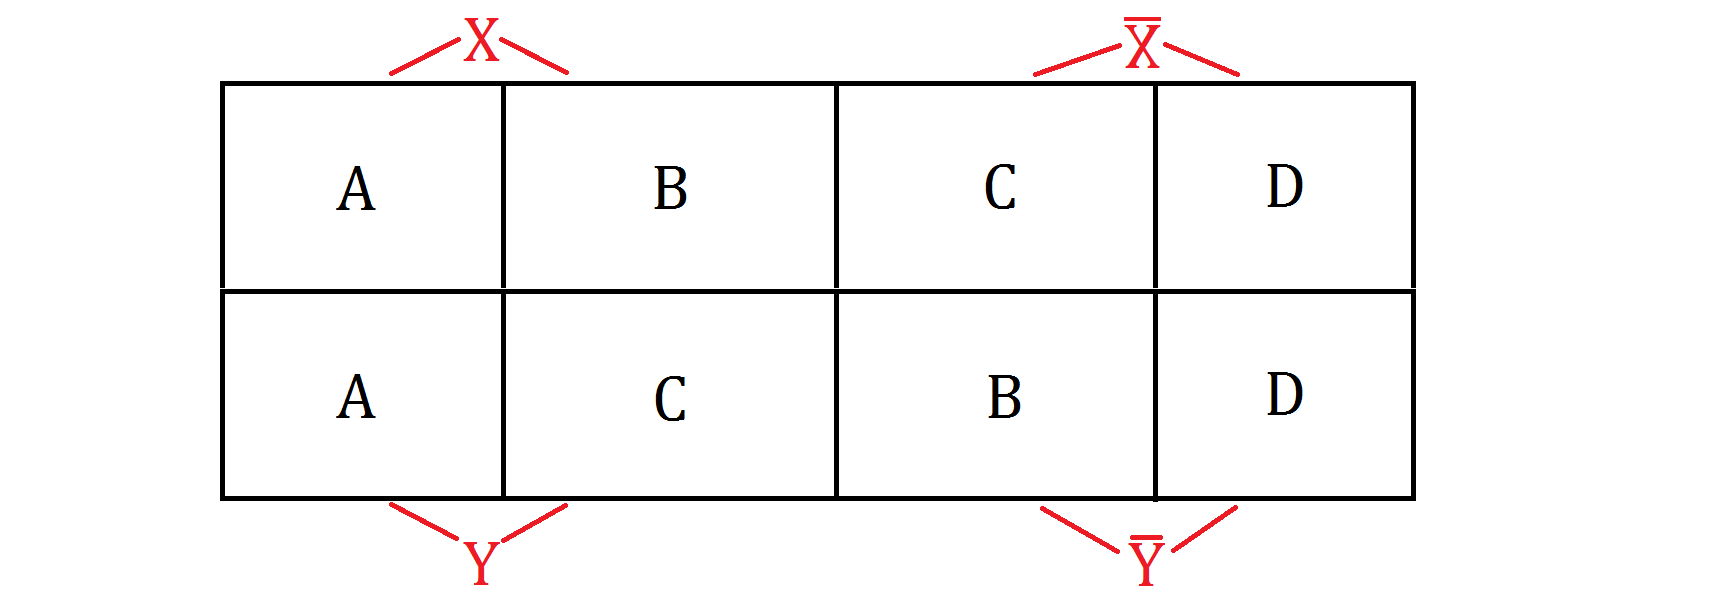
\includegraphics[width=140mm]{pic1.png}
	\end{figure}
	
	考虑如下的coupling形式, 我们将$A_x, B_x, C_x, D_x$分别从小到大排序, 用下标表示其中的元素(下标越界时从头开始), $X_x = A_x \cup B_x$, $Y_x = A_x \cup C_x$.

	随机出两个数$a\in[k], b\in[n-k]$, 则第$x$步对$X_x,Y_x$进行如下操作:
	\begin{enumerate}[(1)]
		\item $a \leq i, b \leq k - i$:
				$$X_{x+1} = X_{x} - A_{x}(a) + C_{x}(b)$$
				$$Y_{x+1} = Y_{x} - A_{x}(a) + B_{x}(b)$$
		\item $a > i, b \leq k - i$: 
				$$X_{x+1} = X_{x} - B_{x}(a) + C_{x}(b)$$
				$$Y_{x+1} = Y_{x} - C_{x}(a+1) + B_{x}(b+1)$$
		\item $a \leq i, b > k - i$:
				$$X_{x+1} = X_{x} - A_{x}(a) + D_{x}(b)$$
				$$Y_{x+1} = Y_{x} - A_{x}(a) + D_{x}(b)$$
		\item $a > i, b > k - i$: 
				$$X_{x+1} = X_{x} - B_{x}(a) + D_{x}(b)$$
				$$X_{x+1} = X_{k} - C_{x}(a) + D_{x}(b)$$
	\end{enumerate}

	可以证明这样的coupling对应的边际分布是与原问题相同的.

	除了(3), 其它几种操作后, $|X\cap Y|$都会上升至少$1$, 在操作(3)后, $|X\cap Y|$不变.

	这样, 我们可以计算使得$X_t = Y_t$的最小的$t$, 设$T_i$为$|X\cap Y| = i$的最早时间, 则有(第一个不等式由几何分布的期望得出, 不是等号的原因是操作(2)使$|X\cap Y|$增长超过$1$):

	\begin{eqnarray*}
		E[T_{i+1}] & \leq & E[T_{i}] + \frac{1}{1 - \frac{i}{k}\times\frac{n-2k+i}{n-k}} \\
				   & \leq & E[T_{i}] + \frac{1}{1 - \frac{i}{k}}\\
				   & \leq & E[T_{i}] + \frac{k}{k - i}
	\end{eqnarray*}

	解得$$E[T_n] \leq \sum_{i=0}^{k - 1} \frac{k}{k-i} = k \log k + O(1)$$

	为了求出\textit{mixing time}, 
	\begin{eqnarray*}
		\forall X, Y & & \\
		\Delta(t) 	& \leq & \textit{Pr}\left[
			X_t\not= Y_t
		\right]	 \\ 
		& = & \textit{Pr}\left[T_n > t\right] \\
		&\leq& \frac{k\log k + O(1)}{t} 
	\end{eqnarray*}

	令其$\leq\frac{1}{2e}$, 求出:

	$$\tau_{mix} = 2ek\log k + O(1) = O(n\log k)$$
\end{enumerate}

\section*{Acknowledgements}
感谢游宇榕在第五题给予的提示, 让我的上界直接降低了一个阶.
\end{document}